\chapter{Transistor en zona de corte}
En esta actividad de simulación se nos encomendó la tarea de analizar el comportamiento del transistor NPN en configuración emisor-común implementando en el simulador LTSpice el siguiente circuito  

\begin{minipage}[b]{0.7\textwidth}
        \centering
        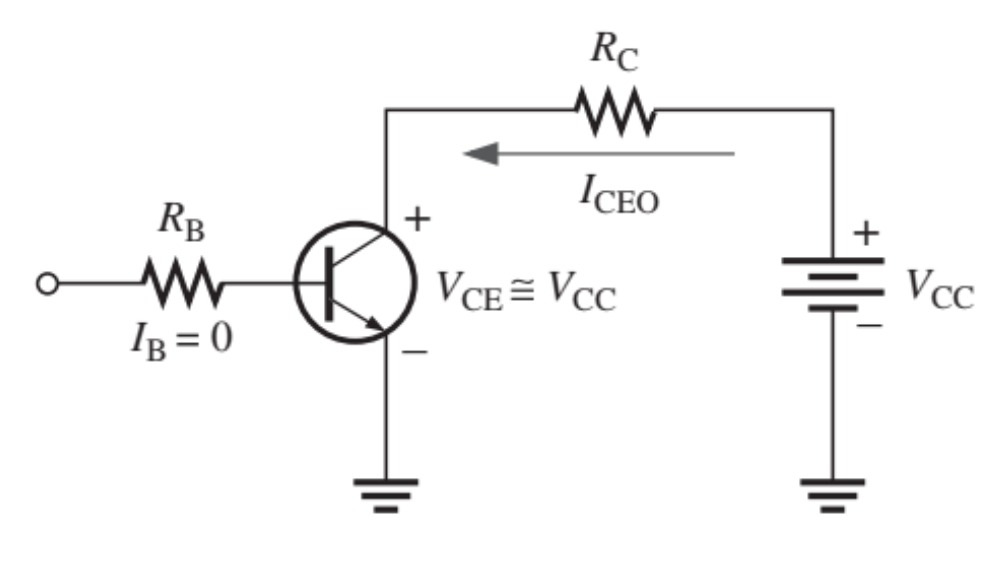
\includegraphics[width=\textwidth]{images/zona_corte.jpg}}
        \caption*{(Operación de un BJT que muestra el flujo de electrones.}
    \end{minipage}
    \hfill
    como se puede observar, este circuito no se tiene ninguna fuente de energía en la base. Por lo tanto, el transistor no
podrá polarizar en directa la unión BE (IB=0) y por consiguiente no se promoverá la
circulación de corriente en el circuito de salida (IC). En esta condición, sin embargo existe una cantidad muy pequeña de corriente de fuga en el colector, ICE0, debido principalmente a portadores

\subsection{Actividad de simulacion}

\begin{figure}[H]
  \centering
  \begin{tikzpicture}
    \begin{axis}[
        width=12cm,
        height=8cm,
        xlabel={$t$ [s]},
        ylabel={$I$ [nA]},
        grid=both,
        minor tick num=1,
        scaled ticks=false,
        xmax=1, xmin=0,
        ymin=1.3, ymax=1.4,
        ytick={1.34, 1.35, 1.36, 1.37, 1.38},
      ]
      \addplot[
        color=red,
        mark=none,
        thick,
      ] table[
        col sep=tab,
        header=true,
        x index=0,
        y index=1
      ] {simulaciones/trans_corte.txt};
      \addlegendentry{$I_{CE0}$}
    \end{axis}
  \end{tikzpicture}
  \caption{Circulacion de la corriente de fuga en el colector.}
\end{figure}

\begin{lstlisting}[style=ltspice, caption={Parámetros de simulación LTspice}]
.tran 1
.MODEL BC548B NPN(IS=1.95E-14 ISE=1.31f ISC=1.00E-13 XTI=3.00 BF=2.90E2 BR=2.42 IKF=1.80E-1 IKR=1.00 XTB=1.5 VAF=9.17E1 VAR=2.47E1 VJE=6.32E-1 VJC=3.39E-1 RE=1.00 RC=1.73 RB=2.65E1 RBM=1.00E1 IRB=1.00E1 CJE=1.33E-11 CJC=5.17p FC=9.00E-1 NF=9.93E-1 NR=1.20 NE=1.32 NC=2.00 MJE=3.26E-1 MJC=3.19E-1 TF=6.52E-10 TR=0 ITF=1.03 VTF=1.65 XTF=1.00E2 EG=1.11 VCEO=30 ICRATING=100m MFG=PHILIPS)
\end{lstlisting}

\subsection{Conclusión}
\newpage
